\documentclass[a4paper]{article}
\usepackage[utf8]{inputenc}
\usepackage{amsmath}
\usepackage{esint}
\usepackage{tabstackengine}
\usepackage[colorlinks,linkcolor=blue]{hyperref}
\usepackage{xeCJK}
\usepackage{mathrsfs}
\usepackage{commath}
\usepackage{graphicx}
\graphicspath{{../resources/figure/eng/}}
\usepackage{vowel}
\usepackage{float}
%%%% 下面的命令重定义页面边距,使其符合中文刊物习惯 %%%%
\addtolength{\topmargin}{-54pt}
\setlength{\oddsidemargin}{0.63cm}  % 3.17cm - 1 inch
\setlength{\evensidemargin}{\oddsidemargin}
\setlength{\textwidth}{14.66cm}
\setlength{\textheight}{24.00cm}    % 24.62

%%%% 段落首行缩进两个字 %%%%
% \makeatletter
% \let\@afterindentfalse\@afterindenttrue
% \@afterindenttrue
% \makeatother
% \setlength{\parindent}{2em}  %中文缩进两个汉字位

% 段首不缩进
\setlength{\parindent}{0pt}
%%%% 下面的命令设置行间距与段落间距 %%%%
\linespread{1.4}
% \setlength{\parskip}{1ex}
\setlength{\parskip}{0.5\baselineskip}

\title{英语学习方法}
\author{Crosstyan}
\begin{document}
\maketitle
\section{简介}
目前的英语教学流派大体可以被分为
\begin{itemize}
  \item 着重于教授语法, 让学生死记硬背以达到应试的目的, 着重于读写方面的训练的\textbf{语法翻译法}. 
  \item 强调像幼儿时期一样学习语言, 通过大量的沉浸在目标语言的环境中而自然\textit{获取}的\textbf{二语习得}
\end{itemize}
\par 当然, 我个人觉得最好的学习方式就是将两者结合起来. 有一定的语法基础之后再通过大量地沉浸来达到事倍功半的效果, 然后沉浸的结果再反馈回对语法知识点的理解之中. 
\section{国际音标 (IPA)}
标识世界上所有语言, 当然也包括英语. 英语所用的国际音标的一部分被称为英语国际音标. 
\begin{quote}
  \textit{一个很优秀的学者,用英语读文献、做研究没有任何问题,但是口头交流能力就差了很多。因此,想要提高口语能力,就要训练口语表达。}
\end{quote}
\subsection{元音}

\begin{figure}[H]
\centering
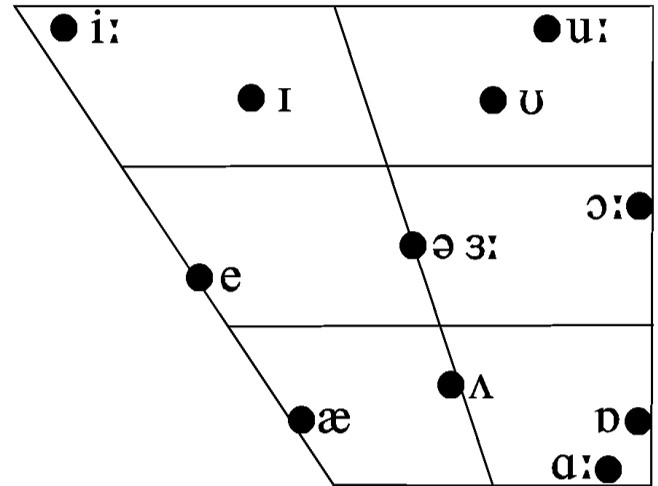
\includegraphics[width=0.33\textwidth]{vowel.jpg}
\caption{元音}
\end{figure}

% % Table generated by Excel2LaTeX from sheet 'Sheet2'
% \begin{table}[H]
%   \centering
%   \caption{Add caption}
%     \begin{tabular}{cc}
%     IPA   & Examples \\
%     ɑː    & PALM, bra \\
%     ɒ     & LOT, blockade \\
%     æ     & TRAP, tattoo \\
%     aɪ    & PRICE, pie \\
%           &  \\
%     aʊ    & MOUTH, how \\
%           &  \\
%     ɛ     & DRESS, prestige \\
%     eɪ    & FACE \\
%           &  \\
%     ɪ     & KIT, historic \\
%     iː    & FLEECE, pedigree, idea \\
%           &  \\
%     oʊ    & GOAT \\
%     ɔː    & THOUGHT \\
%           &  \\
%     ɔɪ    & CHOICE \\
%           &  \\
%     ʊ     & FOOT \\
%     uː    & GOOSE, cruel \\
%           &  \\
%     ʌ     & STRUT, untidy, justiciable \\
%     \end{tabular}%
%   \label{tab:addlabel}%
% \end{table}%

\subsection{辅音}
\begin{figure}[H]
\centering
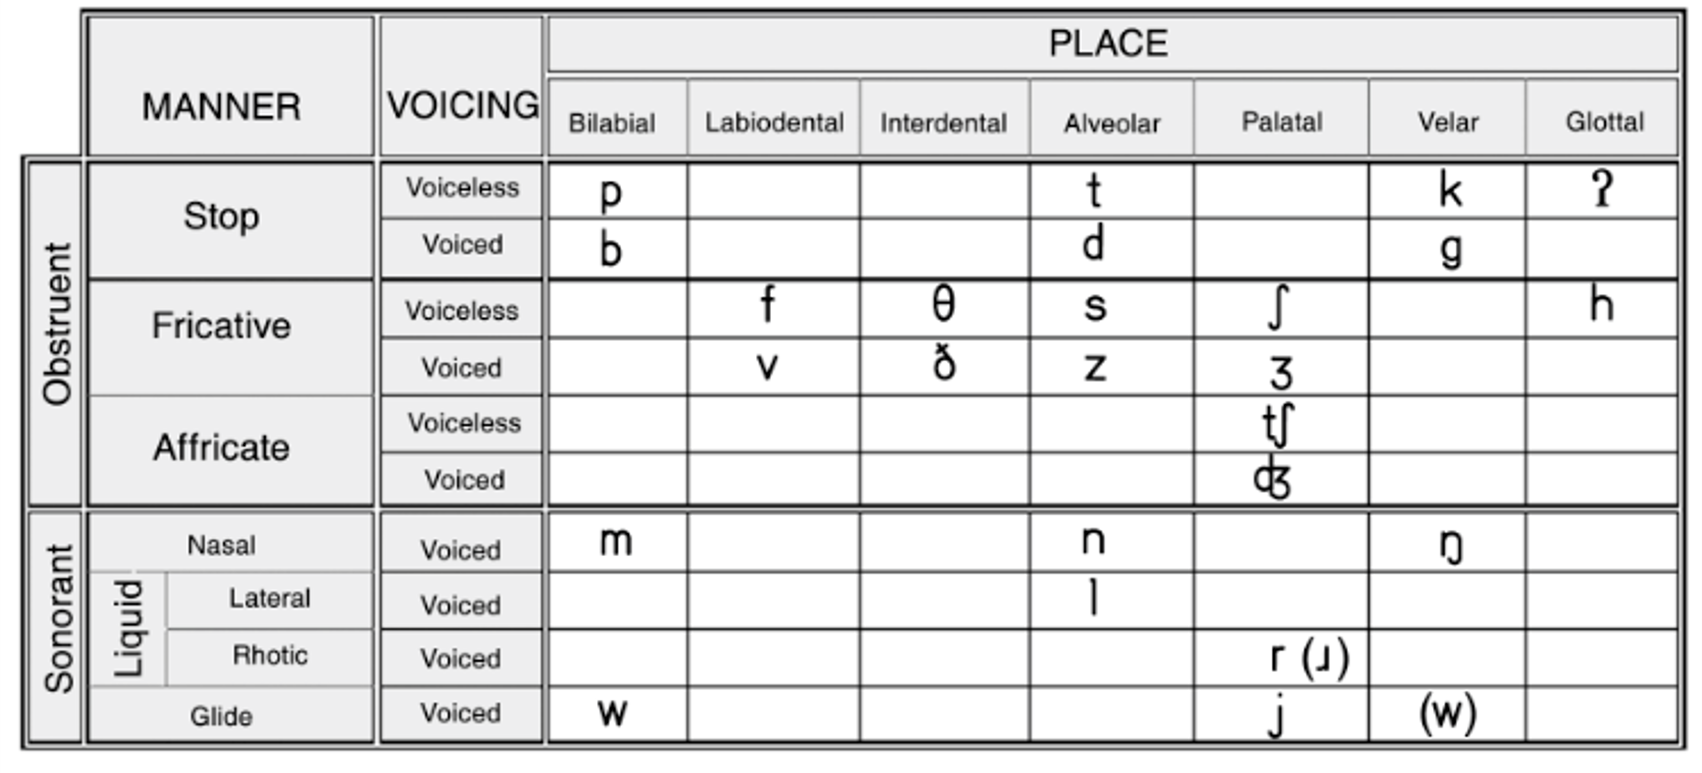
\includegraphics[width=1\textwidth]{cons.png}
\caption{辅音}
\end{figure}
% % Table generated by Excel2LaTeX from sheet 'Sheet1'
% \begin{table}[H]
%   \centering
%   \caption{辅音表}
%     \begin{tabular}{c|c}
%     IPA   & Examples \\
%     b     & buy, cab \\
%     d     & dye, cad, ladder \\
%     dj    & dew \\
%     dʒ    & giant, badge \\
%     ð     & thy, breathe, father \\
%     f     & fan, leaf \\
%     ɡ     & guy, bag \\
%     h     & high, ahead \\
%     hw    & whine \\
%     j     & yes, hallelujah \\
%     k     & sky, crack \\
%     l     & lie, sly, gal \\
%     lj    & lute \\
%     m     & my, smile, cam \\
%     n     & nigh, snide, can \\
%     nj    & new \\
%     ŋ     & sang, sink, singer \\
%     p     & pie, spy, cap \\
%     r     & rye, try, very \\
%     s     & sigh, mass \\
%     sj    & consume \\
%     ʃ     & shy, cash, emotion \\
%     t     & tie, sty, cat, latter \\
%     tj    & tune \\
%     tʃ    & China, catch \\
%     θ     & thigh, math \\
%     θj    & enthuse \\
%     v     & vine, leave \\
%     w     & wine, swine \\
%     z     & zoo, has \\
%     zj    & Zeus \\
%     ʒ     & pleasure, beige \\
%     \end{tabular}%
%   \label{tab:addlabel}%
% \end{table}%
\begin{quote}
  \textit{将输入和输出两方面结合。输入时,在听到一个目的语母语者发出该音节时,不光听辨发音,也要关注说话人的口型、面部表情;如果能看到共鸣腔(口、鼻、咽三腔)以及舌位的立体图就更好了。现在有很多软件和在线课程在教发音时是可以做到这一点的。这样的输入是全面的,也就是从学习者的听感感知和对该音的发音原理都输入了。
  }
  \par
  \textit{为什么要这样?因为很多学习者发不对音,并不是他发不出,而是对他的语音表征系统来说,这两个音在他听来是一样的,这是所谓的「语音的主观性」造成的。在不同的社会环境下成长的人对相同的语音形象会有不同的感知结果。比如,外国人学习汉语时,他们根据自己的母语语音知识去感知中文的语音形象,并不认为自己的中文发音有什么不对,在他们的主观感知中,他们认为发出「窝们歪果仁」和「我们外国人」是没有区别的,所以他们一直这样说,但是作为中国人我们觉得区别非常明显,这也是我们的语音主观性所主导的。再比如 China 的 Ch,中国人容易发成舌面音,但是其实这是一个舌缘音
  }
  \par
  \textit{我们可能并没有注意到外国人发 China 的时候有什么不对,也不觉得自己发音时候有什么不对,由于舌面音的 Ch 和舌缘音的 Ch 并不会造成意义的区别,所以大部分人也不会关注;外国人可能只觉得我们发音奇怪,但是说不出为什么。
 }
 \par
 \textit{所以,要用图音结合的方法矫正口音,同时也要看到自己的问题,因为我们听感上已经无法辨别,必须要靠更精细的技术替代我们的耳朵来进行矫正。这一条很难实现,尤其是看到自己的共鸣腔和舌位立体图,现在恐怕还没有这样的技术,但是看一个母语者的发音口型和立体图,现在还是有很多。可以把自己的发音录下来听一听,和母语者比对一下,这也是有帮助的。}
\end{quote}

\section{语法分析}
以下的概念都是绝大部分语言都共有的 (也就是说掌握了这些内容就可以很快地熟悉世界上任何语言的\textbf{大体框架}, 但也只是框架而已), 为了方便讲解就挑选了其中英语用到的分类. 要掌握一门语言是一件十分困难的事情, 需要大量的沉浸. 当然如果只是应试的话当然背语法概念是效率最高的方法, 可是这样学习是十分枯燥的, 孩子的接受程度也不高. 

\subsection{句子成分}
\begin{quote}
  \textit{一个英语句子有且仅有一个谓语动词,其他动词要用非谓语动词或从句的形式。}
\end{quote}
\subsubsection{主语}
动作的执行者, 或者我们所谈论的主题. 
\subsubsection{谓语}
做了什么样的动作, 是一个句子不可或缺的成分. 
\subsubsection{宾语}
动作的承受者, 和表语(主语补语)不同. 
\subsubsection{定语}
可以理解为是「泛形容词」, 用于修饰名词或者代词之类的. 
\subsubsection{状语}
可以理解为是「泛副词」, 用于修饰动词或者整个句子. 
\subsubsection{补语}
\paragraph{主语补语}
又被称为表语, 对主语的补充说明. 存在于「主系表」的语法结构中. \\
其中的系表示系动词(也属于谓语), 表就是表语(又被称为主语补语). 
\paragraph{宾语补语}
对宾语的补充说明. 存在于「主谓宾宾补」的语法结构中. \\
字典一般会以
$$\text{某动词}\;sb/sth\;(adj./to\;do/doing)$$
标识. 其中$sb/sth$就是该动词的宾语, 后面的部分就是宾补 (可以以形容词, 动词的不定式, 现在分词或者过去分词充当该成分). 
\begin{quote}
  \textit{如果是要判断某个词组是“后置定语”还是“宾语补足语”:这个时候要看该部分的存在是否会影响谓语的含义。\\
  定语和补语是不在一个层次上的。定语在词组的层面上,而补语在分句的层面上。}
\end{quote}
\subsection{词性}
\begin{itemize}
  \item 名词 $noun$
  \item 动词 $verb$
  \item 代词 $pronoun$
  \item 形容词\footnote{形容词修饰名词} $adjective$
  \item 副词\footnote{副词修饰动词或者形容词或者整个句子} $adverb$
  \item 介词 $preposition$
  \item 连词 $conjunction$
\end{itemize}
\subsubsection{名词}
\begin{itemize}
  \item 可数 Countable $[C]$ 与 不可数 Uncountable $[U]$
  \item 单数 Singular $[sing.]$ 与 复数 Plural $[pl.]$ 
\end{itemize}
规则复数变化加s, 不规则变化查字典. 如何知道一个词可数还是不可数? 查字典. 
\subsubsection{动词}
\begin{itemize}
  \item 不及物 Intransitive $[I]$ 及物 Transitive $[T]$
  \item 不定式 (一般在语法上就是$to+\text{动词原形}$)
  \item 过去式
  \item 过去分词 (与过去式区分, 用于完成时以及被动语态)
  \item 现在分词 (俗称ing形式)
\end{itemize}
\paragraph{助动词\protect\footnote{auxiliary verb}} 助动词和实义动词共同作用. 分为基本助动词, 情态助动词\footnote{modal verbs}(简称情态动词)和半助动词. 
\subparagraph{基本助动词}
基本助动词用于表征时态, 往往没有实际意义, 需要和实义动词共同表示意思
\begin{itemize}
  \item be
  \item have
  \item do
\end{itemize}
\subparagraph{情态助动词} 结合实义动词表征一定意义
\begin{itemize}
  \item can/could
  \item may/might
  \item will/would
  \item should/shall
  \item must
  \item ought to
  \item dare
  \item need
  \item used to 
  \item had better
\end{itemize}
\subparagraph{半助动词} 同情态助动词
\begin{itemize}
  \item have to 
  \item seem to
\end{itemize}
\paragraph{系动词\protect\footnote{linking verb, 即联系动词}}
be动词, become, 或者表示感官的词(看起来, 听起来, 闻起来). 构成主系表结构. 
\subsubsection{形容词与副词}
都有比较级, 单音节词加$er$或者$est$, 多音节词用$more$或者$less$来修饰. 
一般来说形容词后面加$ly$可以化为形容词. 详细构词法与词根词缀(在字典附录). 
\subsection{五大句型}
\begin{itemize}
  \item 主谓 (S-V)
  \item 主谓宾 (S-V-O)
  \item 主系表 (S-V-SC)
  \item 主谓宾宾补 (S-V-O-OC)
  \item 主谓双宾语 (S-V-DO\footnote{直接宾语 (direct object)}-IO\footnote{间接宾语 (indirect object)})
\end{itemize}
\subsection{时态}
助动词加实义动词表征时态
\begin{figure}[h]
\centering
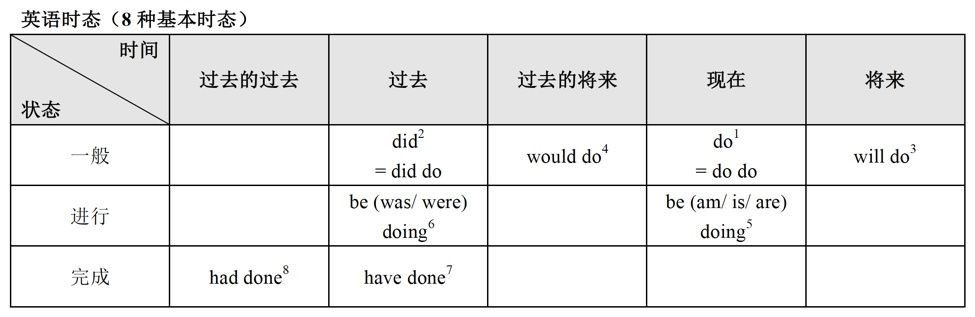
\includegraphics[width=1\textwidth]{tense1.jpg}
\caption{基本时态}
\end{figure}
\begin{figure}[h]
\centering
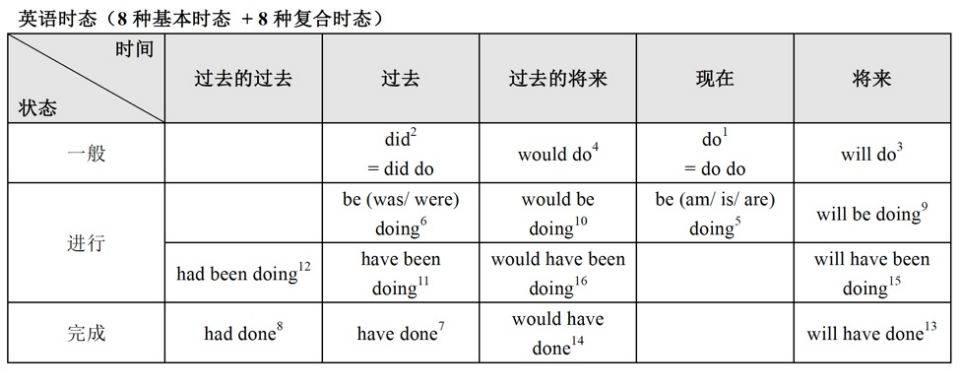
\includegraphics[width=1\textwidth]{tense2.png}
\caption{复合时态}
\end{figure}
\begin{figure}[h]
\centering
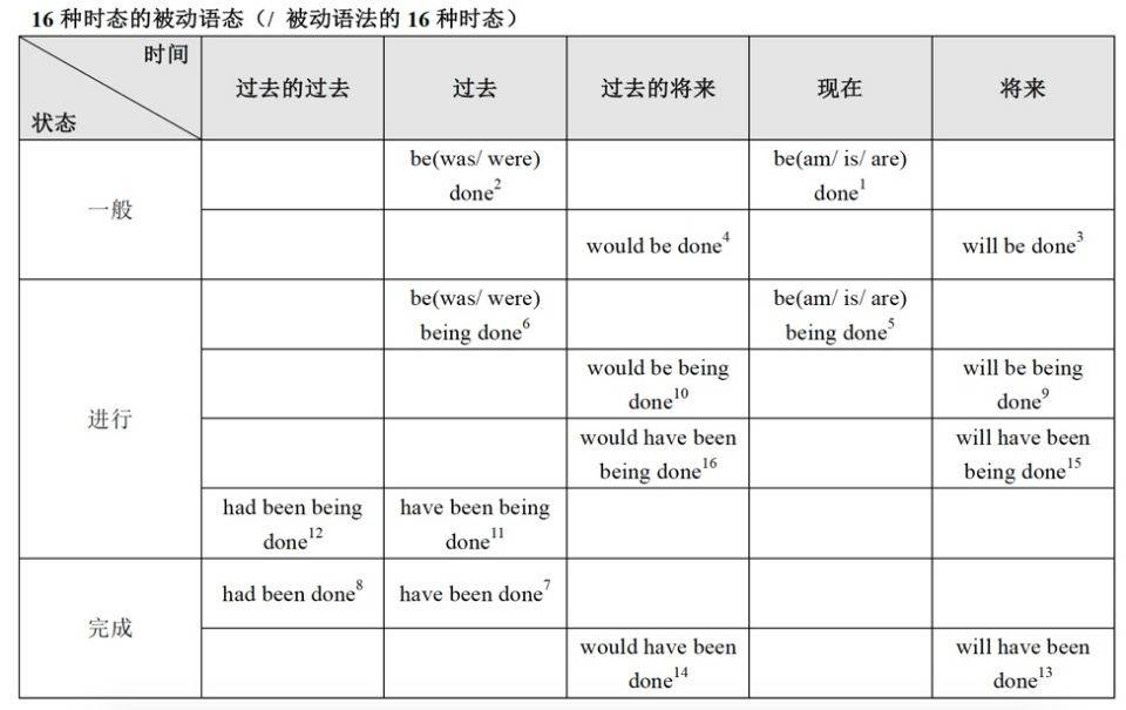
\includegraphics[width=1\textwidth]{tense3.jpg}
\caption{包括被动语态的复合时态}
\end{figure}
\subsection{从句}
一个复合句可以被分为主句和从句, 一个句子必须要有主句, 只有主句的句子就被称作简单句; 有主句和从句的被称作复杂句. \\
$$\text{连词 }\;conj.+\text{从句}$$
that在作为连词的时候常常会被省略(在先行词作为从句宾语的定语从句和宾语从句之中). \\
除了谓语, 其他句子成分都会有一个相对应的从句. 
\subsubsection{状语从句}
随着连词(引导词)的不同, 可以分为以下不同的从句类型. 
\begin{itemize}
  \item 时间状语从句
  \item 地点状语从句
  \item 原因状语从句
  \item 条件状语从句
  \item 让步状语从句
  \item 目的状语从句
  \item 结果状语从句
  \item 方式状语从句
  \item 比较状语从句
\end{itemize}
具体参考基础知识手册「状语从句」一节
\subsubsection{主语从句}
充当主语的从句, 常常由$that,what$引导
\subsubsection{宾语从句}
充当宾语的从句, 其中宾语可以是双宾语中的间宾. 
\subsubsection{定语从句}
充当定语的从句, 被修饰的词称为先行词. 先行词在宾语从句中被省略. 由此可分为
\begin{itemize}
  \item 先行词充当定语从句主语 (从句无主语)
  \item 先行词充当定语从句宾语 (从句无宾语)
\end{itemize}
\section{如何积累单词}
\begin{quote}
  \textit{具体方法很多,典型的方法就是:多看、多听、多见。所谓见多识广,当你接触了大量的听力和阅读训练,单词出现的语境也就会更丰富和全面,大脑的统计学习提取也就更精确,这是我上文中提到的单词的内隐学习\footnote{就是二语习得理论中依靠阅读和听力潜移默化地学习, 而不使用死记硬背单词和语法点的方式}。当然,我们也可以把这个行为变成有意识的、外显的学习行为,毕竟,当我们付出注意力的时候,单词留在大脑上的痕迹也会更加长久。}
\end{quote}
在阅读中积累单词, 每当遇到一个不会的单词, 你可以去试着猜测它的意思. 但是如果句子按照你猜测的意思读不通顺, 或者在文章出现了很多次 (证明这是一个重点单词), 那么你就必须去查字典. 
\par
当查字典之后, 将这个单词记录在一本专有的笔记本里面, 形成自己的生词本. 其中每个条目要包含的项目有
\begin{itemize}
  \item 单词拼写
  \item 音标
  \item 词性 (很重要)
  \item 意思 (初学者可以写中文释义, 进阶之后只写英文释义)
  \item 常见用法 (若是动词标明是否及物, 是否接双宾语或者宾补) (若是名词则注意是否可数)
  \item 例句 (可选, 帮助理解)
\end{itemize}
单词本身和它的意思之间最好不要死记硬背, 而是通过图像, 或者例句, 情景来背. 不要用母语去理解英语单词, 在进阶之后用英语来解释英语单词. 
\begin{quote}
  \textit{我们看到一个陌生单词,看一眼中文意思,很快就能理解一句话的意思了,而且通过这种中英对译的方式也提高了词汇量。但这样学习方式的结果可能是在加重前一章所说的单词的僵化。我们对某些单词的提取总是依赖母语作为媒介而通达,而这种对词汇提取和通达的慢速度直接影响我们加工英语的水平。也就是说,我们可以通过中英对译的方法能达到某个水平,可是再往上提高就难了。}
\end{quote}
\begin{quote}
  \textit{最后的建议是,单词学习,不要以单词量的扩大为主要目的,也不要贪快。单词学习非一日之功,短时背会的单词,在大脑中都是「死单词」。每一个单词都是一个小宇宙,是立体的、多样的,只有我们锲而不舍,遵循合理的方法,才能让它爆发。}
\end{quote}
\section{如何沉浸}
\subsection{推荐的资源}
在通过看动画片, 或者美剧英剧的时候, 绝对, 绝对\textbf{不能看中文字幕}. 在沉浸的时候\textbf{切忌出现任何中文内容}. 一般看剧会看两遍: 第一遍是大概这个剧集讲了什么故事, 如果有不认识的词, 但是觉得很在意的话, 可以暂停去查字典; 第二遍就是精听, 尽量弄明白里面的表达, 当然还是依靠字典, 还有你的耳朵; 当然有条件可以多刷几遍, 能跟着模仿\footnote{使用\href{https://www.bilibili.com/video/BV1bt411W7wF?from=search&seid=7195295628981255603}{史嘉琳教授的回音法}}是最好的. 
\par 可以在Netflix等平台找到带英文字幕的动画片或者剧集. 也可以去听\href{https://learnenglish.britishcouncil.org/general-english/podcasts}{British Council的播客}. 当然百词斩里面的爱阅读或者每日英语听力之类的国产软件\footnote{\href{http://www.aboboo.com/}{Aboboo}似乎是个不错的推荐}也足够使用了. 
\begin{quote}
  \textit{当你觉得自己发音和母语者真的没区别了或者,如果你找个母语者听一下,他也认为你的发音非常标准,就说明你完成了很重要的一步:已经明白如何准确地发出这个音。但是,这远远不够,因为你发对一次,不代表你能发对一万次,要想形成一个有效的语音表征,需要继续练习,而且每一次练习都要正确,不仅单个音节,放在其他词组里、句子里、语流里,都要达到既准确又足够量。前文提过,知识的建立和技能的获得并不等同,也就是说,知识学会了也只是知识,要达到技能熟练水平,还需要大量、充足的练习。就像你能顺利弹下一首曲子,但是你可能需要练一千次,才能在任何场合都毫无压力地弹完这首曲子。}
\end{quote}
\end{document}